\documentclass[12pt,onecolumn,a4paper]{article}
\usepackage{epsfig,graphicx,subfigure,amsthm,amsmath}
\usepackage{color,xcolor}     
\usepackage{xepersian}
\settextfont[Scale=1.2]{BZAR.TTF}
\setlatintextfont[Scale=1]{Times New Roman}





\begin{document}
\title{گزارش پروژه \lr{Appliance Detection}} 
\author{آریا ابراهیمی، سارا قوام‌پور، ملیکا ذبیحی نیشابوری\\}

\maketitle

\section{مقدمه} 
هدف کلی از این پروژه تشخیص رویداد ها در شبکه مصرفی خانگی می‌باشد. روش ارائه شده در این پروژه مبتنی بر شبکه های عصبی پیچشی 
\footnote{\lr{CNN}}
می‌باشد. در بخش اول به منظور جمع‌اوری داده برای آموزش شبکه، نیاز است تا از جریان مصرفی وسایل نمونه برداری شود. در گام بعدی پیش پردازش های لازم بر‌روی داده های به‌دست آمده انجام می‌شود. سپس شبکه با داده های پیش‌پردازش شده آموزش می‌بیند و در نهایت با وزن های به دست آمده توسط شبکه ذکر شده، برای داده ها به صورت برخط، رویداد های مربوط به وسایل را تشخیص می‌دهد.


\section{جمع‌آوری داده‌}

برای این بخش یک سنسور غیر تهاجمی
\footnote{\lr{Non-intrusive}}
\lr{SCT013}
و بورد 
\lr{Arduino}
مورد استفاده قرار گرفته است. سنسور \lr{SCT013} باید دور یکی از سیم های فاز یا نول قرار بگیرد به صورتی که جهت فلش آن به سمت مصرف کننده باشد. داده‌های مربوط به این سنسور توسط مدار شکل۱ به سیگنال‌های دیجیتال تبدیل شده و در نهایت به عنوان ورودی به \lr{Arduino} داده می‌شود.\\
در این پروژه از داده‌های مربوط به سشوار و اتوی مو استفاده شده است، همچنین برای عمل‌کرد بهتر و قدرت تمایز بیشتر، داده مربوط به عدم رخ‌داد رویداد نیز جمع‌اوری شده است. بدین منظور وسیله‌های انتخاب شده را به یک سه‌راه که فاز و نول آن جدا شده‌است متصل کرده و با خاموش و روشن کردن سه‌راه، جریان مصرفی هر کدام را به دست می‌اوریم.\\
در کد مربوط به \lr{Arduino} از کتابخانه 
\lr{EmonLib}
که مربوط به داده‌های انرژی است استفاده شده است. این کتابخانه در هر ثانیه تقریبا ۵۵۸۸ نمونه می‌گیرد. در این پروژه از ۱۱۲ نمونه برای محاسبه جریان 
\lr{RMS}
استفاده می‌شود. بنابراین در هر ثانیه ۵۰ نمونه متفاوت از جریان \lr{RMS} به دست خواهد آمد.

\begin{figure}
	\centering
	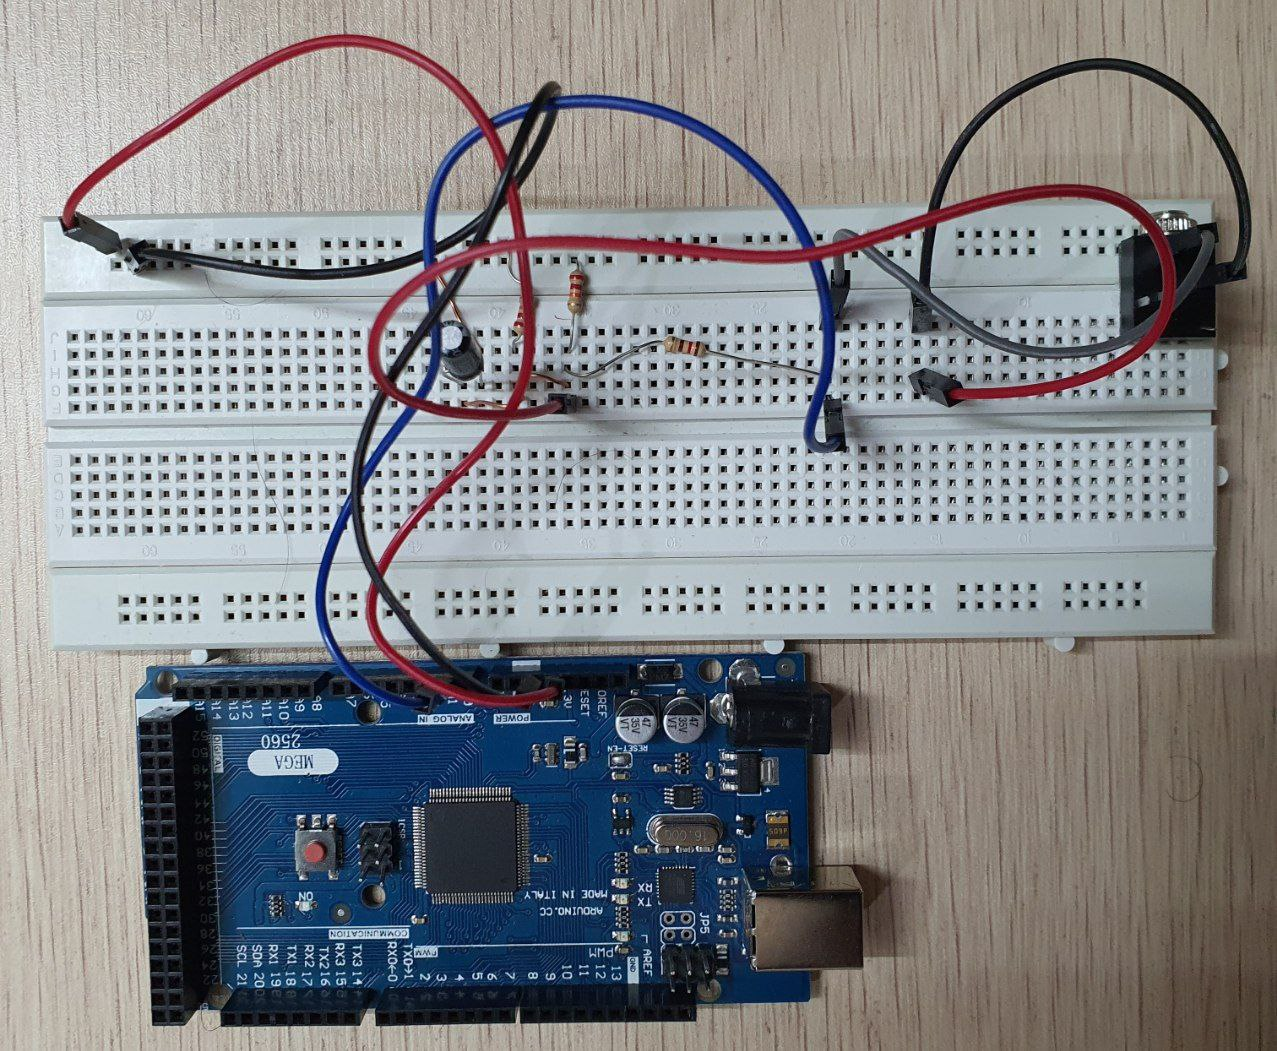
\includegraphics[totalheight=8cm]{Images/1.jpg}
	\caption{مدار استفاده شده برای دریافت داده‌ها و ارسال به \lr{Arduino}}
	\label{fig:verticalcell}
\end{figure}

\section{پیش پردازش}
در این بخش ابتدا مشتق جریان \lr{RMS} محاسبه می‌شود. در یادگیری عمیق، برای کار با داده‌های به فرم سیگنال، مرسوم است که تبدیل فوریه کوتاه مدت سیگنال برای به دست آوردن ویژگی های سیگنال محاسبه شود. 
\lr{Spectogram}
حاصل برای رویداد های خاموش و روشن یکسان است، برای رفع این مشکل اسپکتوگرام های به دست آمده در تابع علامت ضرب می‌شوند. تابع علامت با محاسبه تفاضل دو جریان \lr{RMS} متوالی، صعودی یا نزولی بودن را نشان می‌دهد. مثبت بودن تابع علامت به معنای رویداد روشن شدن است.\\
برای جلوگیری از 
\lr{overfit}
شدن شبکه، از دو مرحله 
\lr{data augmentation}
به منظور افزایش تعداد داده‌ها استفاده شده است. \\
در مرحله اول در زمان دریافت سیگنال‌‌های ورودی، مقدار کمی نویز به آن‌ها اضافه می‌شود. بدین منظور چهار توزیع متفاوت نویز به هر ۵۱۲ نمونه جریان \lr{RMS} اضافه می‌شوند. عکس‌های به دست آمده با اندازه
$32 \times 148$
ذخیره می‌شوند.
\\
در مرحله دوم، چهار برش تصادفی با اندازه 
$32 \times 128$
از تصاویر قبلی جدا می‌شوند. بدین ترتیب از ۵۱۲ نمونه واقعی، ۲۰ تصویر تشکیل می‌شود.

\begin{figure}
	\centering
	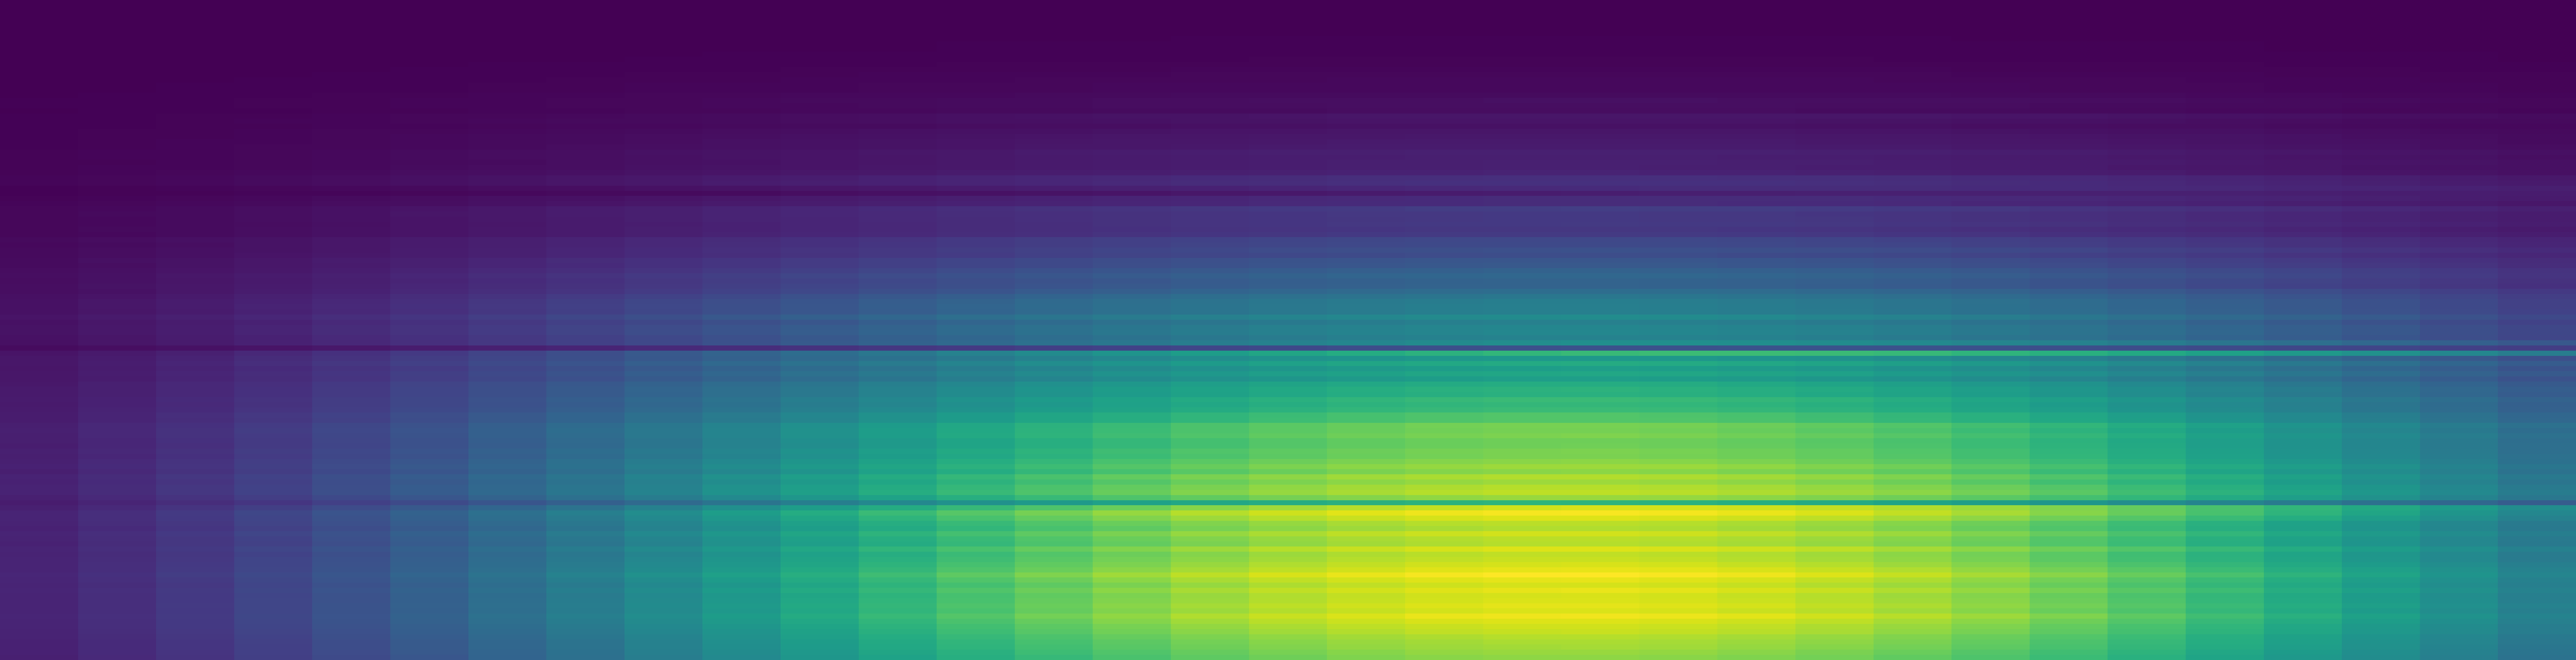
\includegraphics[totalheight=3cm]{Images/2.png}\\
	\vspace{5pt}
	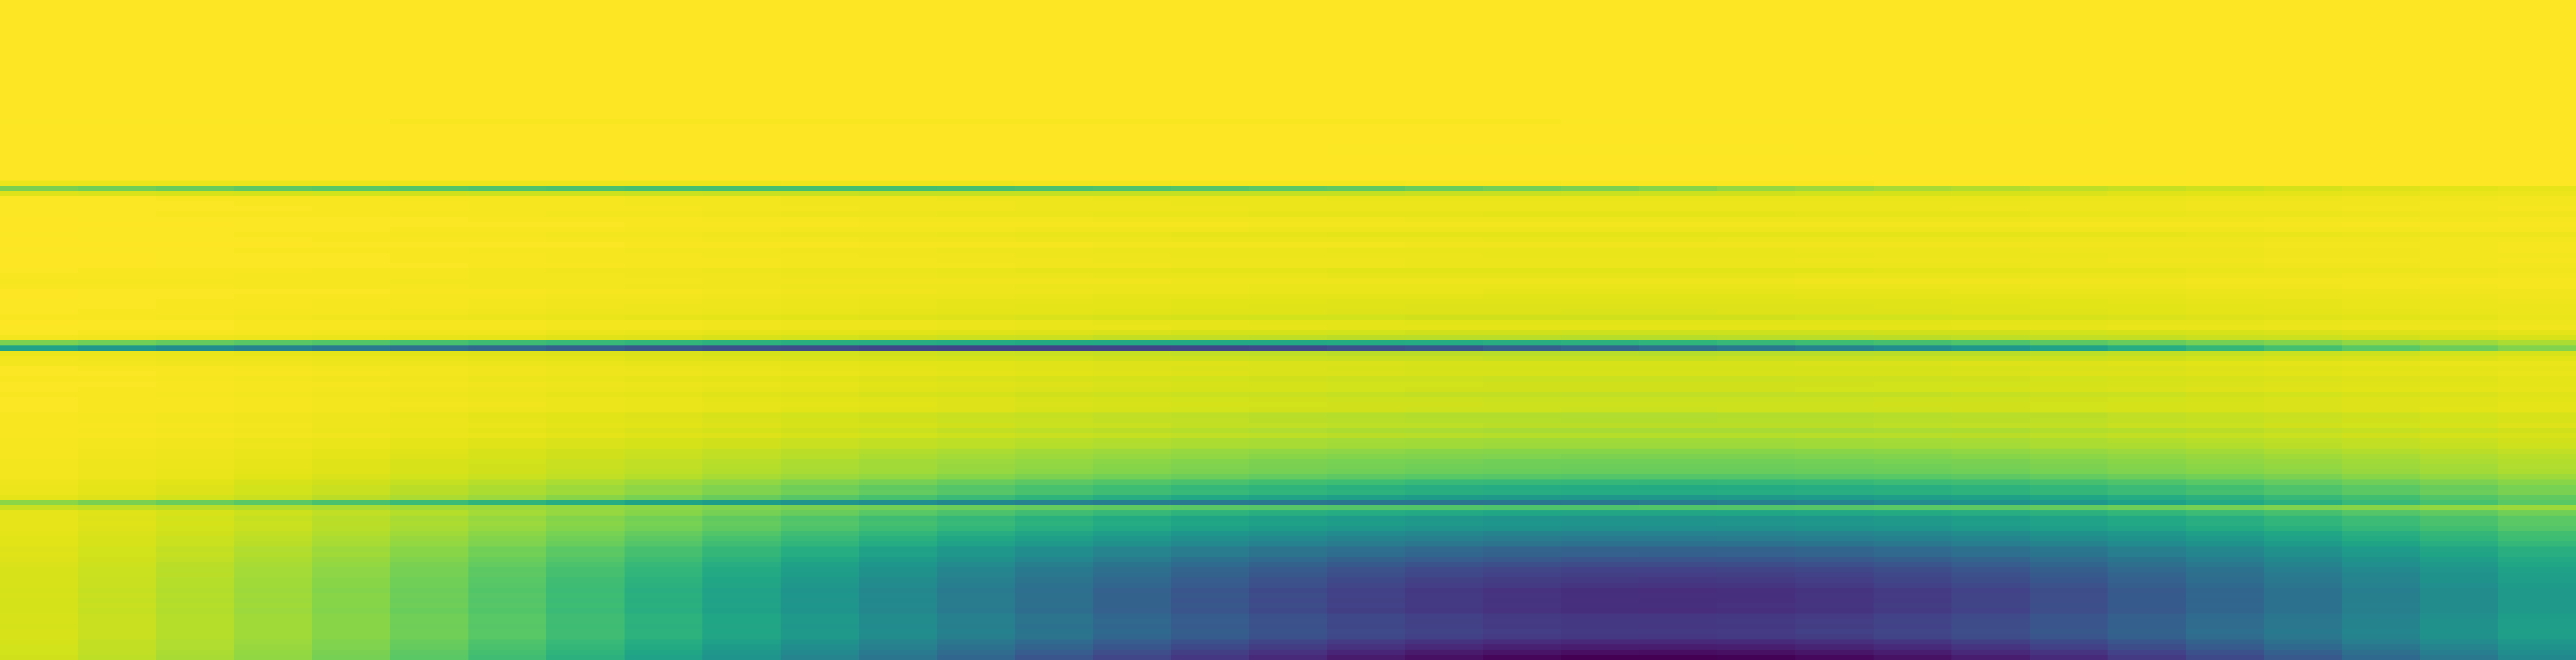
\includegraphics[totalheight=3cm]{Images/3.png}
	\caption{در تصویر بالا،اسپکتوگرام به دست آمده مربوط به رویداد روشن شدن سشوار، و در تصویر پایین اسپکتوگرام مربوط به رویداد خاموش شدن سشوار نمایش داده شده اند. }
	\label{fig:data}
\end{figure}

\section{شبکه عصبی}

ورودی شبکه با سایز 
$32 \times 128$
از لایه های مشخص شده در شکل۳ عبور می‌کند. همچنین از یک لایه 
\lr{Dropout}
برای جلوگیری از 
\lr{overfitting}
استفاده شده است.\\
تعداد کل داده های استفاده شده برای آموزش شبکه ۵۳۸۰ است، که از این مقدار ۴۳۰۴ برای داده های آموزش و ۱۰۷۶ برای داده های اعتبارسنجی استفاده شده است. شبکه با \lr{batch} های با اندازه ۱۲۸ در ۱۵ \lr{epoch} آموزش داده شده است، و به دقت ۹۹.۸ درصد برای داده های آموزش و ۹۹.۵ درصد برای داده های اعتبارسنجی می‌رسد.\\
پس از آموزش شبکه، مدل یادگیری شده ذخیره می‌شود تا در مرحله تست برخط استفاده شود. در این گام همانند بخش جمع آوری داده، اسپکتوگرام‌ها را از نمونه های ورودی تشکیل داده و بعد از پیش پردازش به مدل ذخیره شده به عنوان ورودی داده می‌شوند.

\begin{figure}
	\centering
	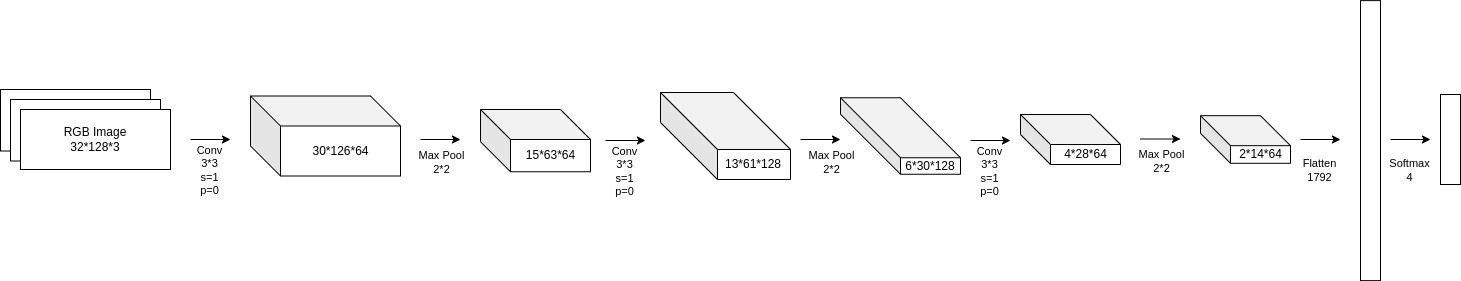
\includegraphics[totalheight=2.7cm]{Images/4.png}\\
	\vspace{5pt}
	\caption{معماری ارائه شده برای شبکه}
	\label{fig:data}
\end{figure}


\section{چالش‌ها و کارهای آینده}
چالش اصلی که در این پروژه وجود دارد جمع‌آوری و آماده سازی داده‌ است. شبکه‌های عصبی عمیق برای یادگیری به داده زیاد نیاز دارند، و جمع آوری داده مورد نیاز در این پروژه ملزم به روشن و خاموش کردن متعدد وسایل می‌باشد که از نظر ایمنی وسایل چالش برانگیز است.\\
چالش بعدی این است که برای برخی از وسایل مانند هیتر و سشوار، اسپکتوگرام های مشابهی به دست می‌آیند که شبکه نمیتواند به خوبی آن‌ها را از هم تمایز دهد. یک راه برای حل این مشکل این است که داده‌های بیشتری جمع آوری شوند که همان‌طور که گفته شد چالش برانگیز است. راه دیگری که میتوان ارائه داد، استفاده از 
\lr{Contrastive Learning}
است این روش بازنمایی ها را به نحوی یادمی‌گیرد که بازنمایی داده های یک کلاس یه هم نزدیک شوند و بازنمایی داده‌ های کلاس‌های متفاوت از یکدیگر دور شوند که باعث افزایش دقت در طبقه بندی می‌شود.


\end{document}